% =====================================================================================
% A-client.tex - PHẦN II của Nguyễn Thành Trung: client Unity
% =====================================================================================

% ---------- Macro đánh số phần tử trên hình HUD ----------------------------------------
\newcommand{\uiN}[3]{\node[circle, fill=uiRed, text=white, inner sep=0pt, minimum size=11pt, font=\tiny\bfseries] at (#1,#2) {#3};}

\PhanLon{II. NỘI DUNG CÁ NHÂN - Phân hệ client Unity.}

\section{Biểu đồ và giao diện nội dung cá nhân thực hiện}
Phân hệ client là nơi các thư viện mạng được đưa vào trò chơi thật. Nhiệm vụ gồm: mở \textbf{điểm nối netcode}
trong mã gameplay một người chơi mà không phá lối chơi gốc; làm cho \textbf{người chơi ở xa hiển thị mượt} (nội suy,
hoạt ảnh, ragdoll cục bộ); làm cho \textbf{người chơi cục bộ phản hồi tức thì} (dự đoán và hoà giải); và xây dựng
\textbf{giao diện} sảnh chờ, HUD, overlay chẩn đoán. Đây cũng là thành viên duy nhất mở Unity Editor.

% -------------------------------------------------------------------------------------
\subsection{Điểm nối netcode trong mã gameplay}
\begin{figure}[H]
\centering
\begin{tikzpicture}[x=1cm, y=1cm,
  cls/.style={draw=cLine, rectangle split, rectangle split parts=2, rectangle split part fill={cBlue,white},
    font=\footnotesize, inner sep=4pt, minimum width=3.4cm},
  inh/.style={draw=cLine, thick, -{Triangle[open, length=3mm]}},
  real/.style={draw=cLine, thick, dashed, -{Triangle[open, length=3mm]}}]
  \node[cls] (actor) at (2.4,0) {\textbf{Actor}
    \nodepart{two}\begin{tabular}{@{}l@{}} - bộ điều khiển nhân vật \\ - chu kỳ cập nhật hình thể \end{tabular}};
  \node[cls] (ac) at (9.6,0) {\begin{tabular}{@{}c@{}}\textit{«trừu tượng»}\\\textbf{ActorController}\end{tabular}
    \nodepart{two}\begin{tabular}{@{}l@{}} - xử lý khai hoả vũ khí \\ - trạng thái ngắm bắn \\ - vận tốc di chuyển \end{tabular}};
  \node[cls] (fps) at (7.2,-3.6) {\textbf{FpsActorController}
    \nodepart{two}\begin{tabular}{@{}l@{}} - nguồn nhập liệu trừu tượng \\ - thiết lập nguồn nhập liệu \end{tabular}};
  \node[cls] (ai) at (12.8,-3.6) {\textbf{AiActorController}
    \nodepart{two}\begin{tabular}{@{}l@{}} AI gốc, chạy trên server \end{tabular}};
  \node[cls] (in) at (7.2,-6.8) {\begin{tabular}{@{}c@{}}\textit{«giao diện»}\\\textbf{IInputSource}\end{tabular}
    \nodepart{two}\begin{tabular}{@{}l@{}} - trục di chuyển \\ - góc nhìn chuột \\ - trạng thái phím bấm \end{tabular}};
  \node[cls] (loc) at (2.6,-10.2) {\textbf{LocalInputSource}
    \nodepart{two}\begin{tabular}{@{}l@{}} bàn phím và chuột \end{tabular}};
  \node[cls] (net) at (7.2,-10.2) {\textbf{NetInputSource}
    \nodepart{two}\begin{tabular}{@{}l@{}} input từ gói mạng \end{tabular}};
  \node[cls] (nul) at (11.8,-10.2) {\textbf{NullInputSource}
    \nodepart{two}\begin{tabular}{@{}l@{}} headless, không input \end{tabular}};
  \node[cls] (rav) at (2.4,-3.6) {\textbf{RemoteActorView}
    \nodepart{two}\begin{tabular}{@{}l@{}} - đồng bộ tư thế, hoạt ảnh \end{tabular}};
  \draw[arr] (actor.east |- ac.west) -- node[lbl, above=2pt]{đọc} (ac.west);
  \draw[inh] (fps.north) -- ++(0,0.6) -| ($(ac.south)+(-0.8,0)$);
  \draw[inh] (ai.north) -- ++(0,0.6) -| ($(ac.south)+(0.8,0)$);
  \draw[arr] (fps.south) -- node[lbl, right=2pt]{dùng} (in.north);
  \draw[real] (loc.north) -- ++(0,0.6) -| ($(in.south)+(-0.8,0)$);
  \draw[real] (net.north) -- (in.south);
  \draw[real] (nul.north) -- ++(0,0.6) -| ($(in.south)+(0.8,0)$);
  \draw[darr] (rav.north) -- node[lbl, left=2pt, align=right]{điều khiển hình thể\\actor ở xa} (actor.south);
\end{tikzpicture}
\caption{Biểu đồ cấu trúc lớp điểm nối: trừu tượng hoá nguồn điều khiển nhân vật}
\label{fig:A-lop}
\end{figure}
Thành phần quản lý nhân vật không phụ thuộc vào nguồn gốc dữ liệu đầu vào. Việc trừu tượng hóa các thao tác điều khiển ra sau giao diện nguồn nhập liệu giúp cùng một bộ điều khiển có thể nhận tín hiệu từ bàn phím (ở client), từ gói tin mạng (ở server) hoặc chế độ tự động không người lái (headless).

% -------------------------------------------------------------------------------------
\subsection{Thứ tự thực thi một khung hình client}
\begin{figure}[H]
\centering
\begin{tikzpicture}[x=1cm, y=1cm]
  \buoc{s1}{(0,0)}{1}{Khởi tạo Client}{Thứ tự ưu tiên: Đọc gói tin mạng, phân phối payload}{cBlue}
  \buoc{s2}{(5.6,0)}{2}{Phương tiện ở xa}{Cập nhật vị trí phương tiện ở xa}{cBlue}
  \buoc{s3}{(11.2,0)}{3}{Nhân vật ở xa}{Nội suy nhân vật ở xa}{cBlue}
  \buoc{s4}{(0,-2.7)}{4}{Bộ hiển thị}{Chiến đấu, mục tiêu, hiệu ứng hình ảnh/âm thanh}{cGreen}
  \buoc{s5}{(5.6,-2.7)}{5}{Input phương tiện}{Xử lý input phương tiện khi đang lái}{cBlue}
  \buoc{s6}{(11.2,-2.7)}{6}{Dự đoán client}{Gửi input, hoà giải khi có snapshot mới}{cGreen}
  \buoc{s7}{(0,-5.4)}{7}{Gameplay gốc}{Nhân vật, vũ khí, giao diện trò chơi}{cOrange}
  \buoc{s8}{(5.6,-5.4)}{8}{Giao diện chẩn đoán}{Hiển thị thông số kết nối và mạng}{cOrange}
  \buoc{s9}{(11.2,-5.4)}{9}{Đối soát chẩn đoán}{So sánh chẩn đoán input và chuyển động}{cGray}
  \draw[arr] (s1) -- (s2); \draw[arr] (s2) -- (s3);
  \draw[arr] (s4) -- (s5); \draw[arr] (s5) -- (s6);
  \draw[arr] (s7) -- (s8); \draw[arr] (s8) -- (s9);
  \draw[arr] (s3.south) -- ++(0,-0.3) -| (s4.north);
  \draw[arr] (s6.south) -- ++(0,-0.3) -| (s7.north);
\end{tikzpicture}
\caption{Chuỗi thứ tự thực thi thành phần client trong một khung hình}
\label{fig:A-thutu}
\end{figure}
Mọi dữ liệu đến được áp dụng \textbf{trước} khi có thành phần nào đọc nó: thành phần giao vận chạy sớm nhất để xác định vai trò mạng trước khi các đối tượng khởi tạo, và các bước chẩn đoán chạy sau cùng.

% -------------------------------------------------------------------------------------
\subsection{Máy trạng thái luồng trò chơi}
\begin{figure}[H]
\centering
\begin{tikzpicture}[x=1cm, y=1cm, st/.append style={text width=2.3cm, minimum width=2.6cm}]
  \node[init] (i) at (1.5,1.5) {};
  \node[st] (boot) at (1.5,0)    {Booting};
  \node[st] (log)  at (5.6,0)    {LoginScreen};
  \node[st] (aut)  at (9.8,0)    {Authenticating};
  \node[st] (lob)  at (14.0,0)   {Lobby};
  \node[st] (rb)   at (14.0,-3.0) {RoomBrowser};
  \node[st] (jr)   at (9.8,-3.0)  {JoiningRoom};
  \node[st] (rl)   at (5.6,-3.0)  {RoomLobby};
  \node[st] (cg)   at (1.5,-3.0)  {ConnectingGame};
  \node[st, fill=cGreen] (im) at (1.5,-6.0) {InMatch};
  \node[st, fill=cOrange] (me) at (5.6,-6.0) {MatchEnd};
  \draw[arr] (i) -- (boot);
  \draw[arr] (boot) -- node[lbl, above=3pt]{Start} (log);
  \draw[arr] ($(log.east)+(0,0.15)$) -- node[lbl, above=3pt]{Log in} ($(aut.west)+(0,0.15)$);
  \draw[arr] ($(aut.west)+(0,-0.15)$) -- node[lbl, below=3pt]{lỗi} ($(log.east)+(0,-0.15)$);
  \draw[arr] (aut) -- node[lbl, above=0.45cm]{LOGIN\_RES} (lob);
  \draw[arr] (lob) -- node[lbl, left=3pt]{Browse rooms} (rb);
  \draw[arr] ($(rb.west)+(0,0.15)$) -- node[lbl, above=3pt]{Join} ($(jr.east)+(0,0.15)$);
  \draw[arr] ($(jr.east)+(0,-0.15)$) -- node[lbl, below=3pt]{lỗi} ($(rb.west)+(0,-0.15)$);
  \draw[arr] (jr) -- node[lbl, above=0.45cm]{ROOM\_JOIN\_RES} (rl);
  \draw[arr] ($(rl.west)+(0,0.15)$) -- node[lbl, above=3pt]{vào trận} ($(cg.east)+(0,0.15)$);
  \draw[arr] ($(cg.east)+(0,-0.15)$) -- node[lbl, below=3pt]{thất bại} ($(rl.west)+(0,-0.15)$);
  \draw[arr] (cg) -- node[lbl, right=3pt]{CONNECT\_ACCEPTED} (im);
  \draw[arr] (im) -- node[lbl, above=0.45cm]{trận kết thúc} (me);
  \draw[arr] (im.south) -- ++(0,-0.8) -| node[lbl, pos=0.12, below=2pt]{mất kết nối} (16.1,0) -- (lob.east);
  \draw[cLine, thick] (me.south) -- ++(0,-0.8) node[lbl, pos=0.5, right=2pt]{Continue / sau 15 s} ;
\end{tikzpicture}
\caption{Máy trạng thái \texttt{GameFlowController}: 10 trạng thái; mọi chuyển trạng thái ngoài bảng đều bị từ chối}
\label{fig:A-trangthai}
\end{figure}

% -------------------------------------------------------------------------------------
\subsection{Giao diện sảnh chờ}
Người chơi đi qua các màn hình theo đúng thứ tự các trạng thái ở Hình~\ref{fig:A-trangthai}: màn hình chính, đăng
nhập, rồi danh sách phòng. Ngoài luồng chơi mạng còn có màn hình luyện tập ngoại tuyến và màn hình cài đặt. Giao diện chẩn đoán sảnh chờ được tích hợp làm công cụ gỡ lỗi nhanh, kích hoạt qua phím tắt Shift+F2.

\begin{figure}[H]
\centering

\includegraphics[width=0.9\textwidth]{image/main-menu.png}
\caption{Màn hình chính: chơi mạng (Multiplayer), luyện tập ngoại tuyến, cài đặt và thoát}
\label{fig:A-menu}
\end{figure}

\begin{figure}[H]
\centering
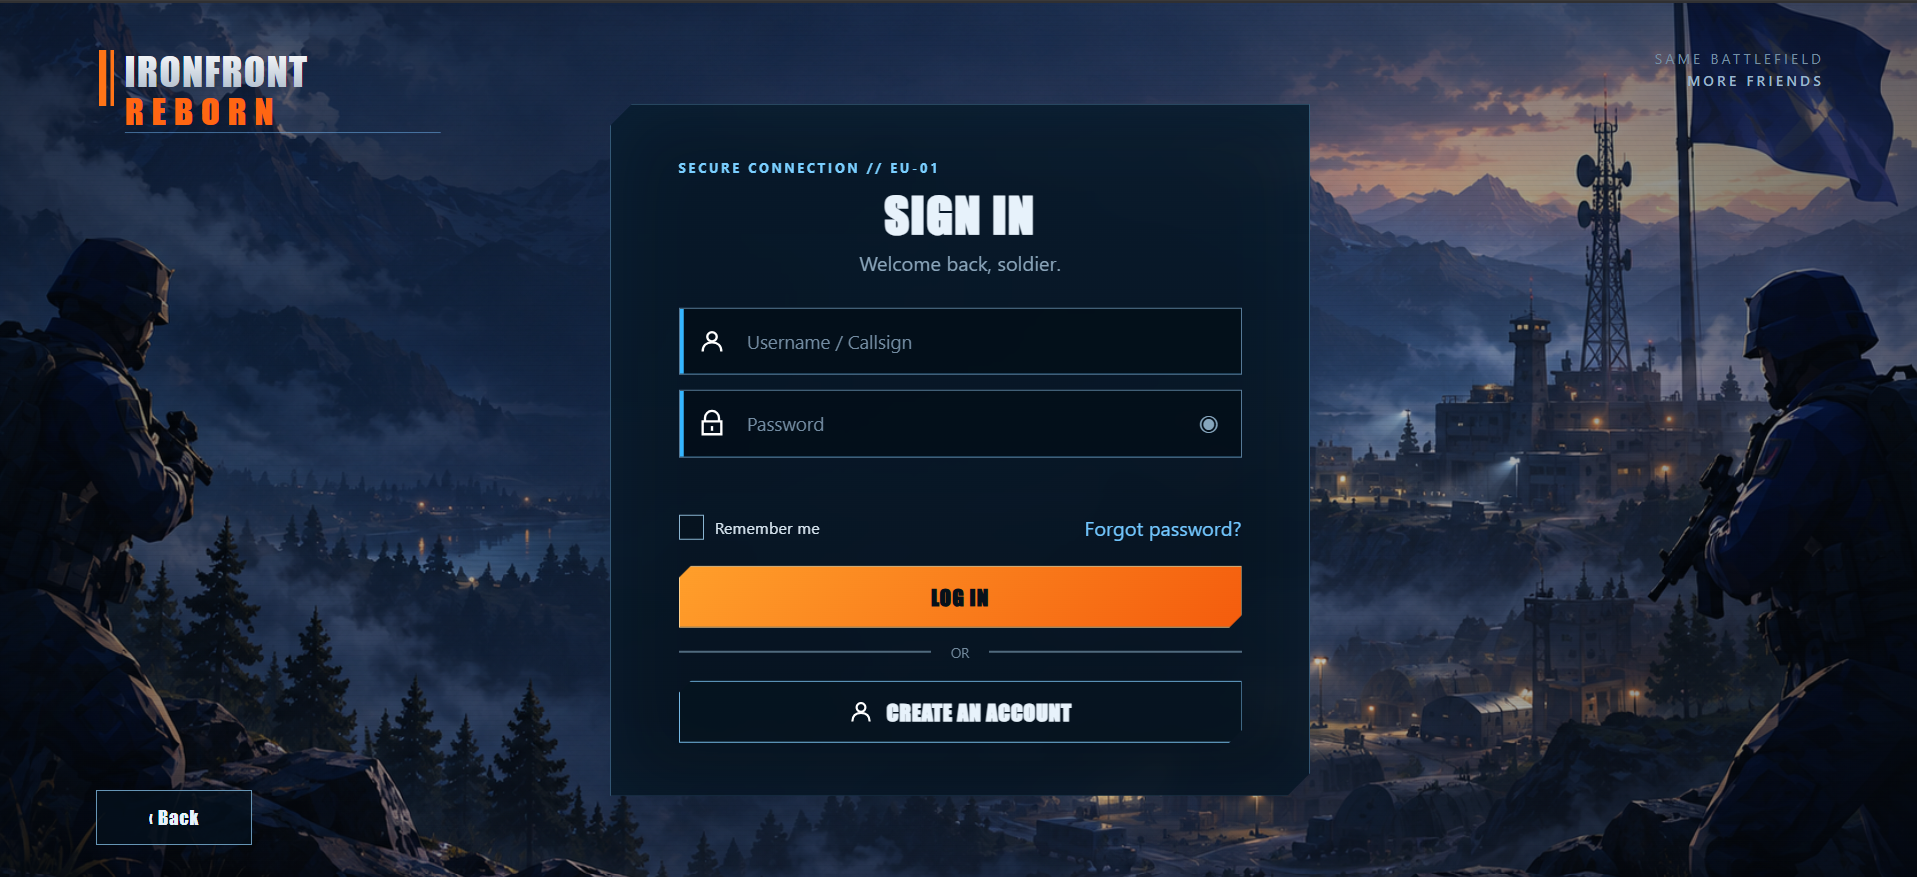
\includegraphics[width=0.9\textwidth]{image/login-screen.png}
\caption{Màn hình đăng nhập (trạng thái \texttt{LoginScreen} / \texttt{Authenticating}): tên đăng nhập, mật khẩu,
tạo tài khoản mới}
\label{fig:A-dangnhap}
\end{figure}

\begin{figure}[H]
\centering
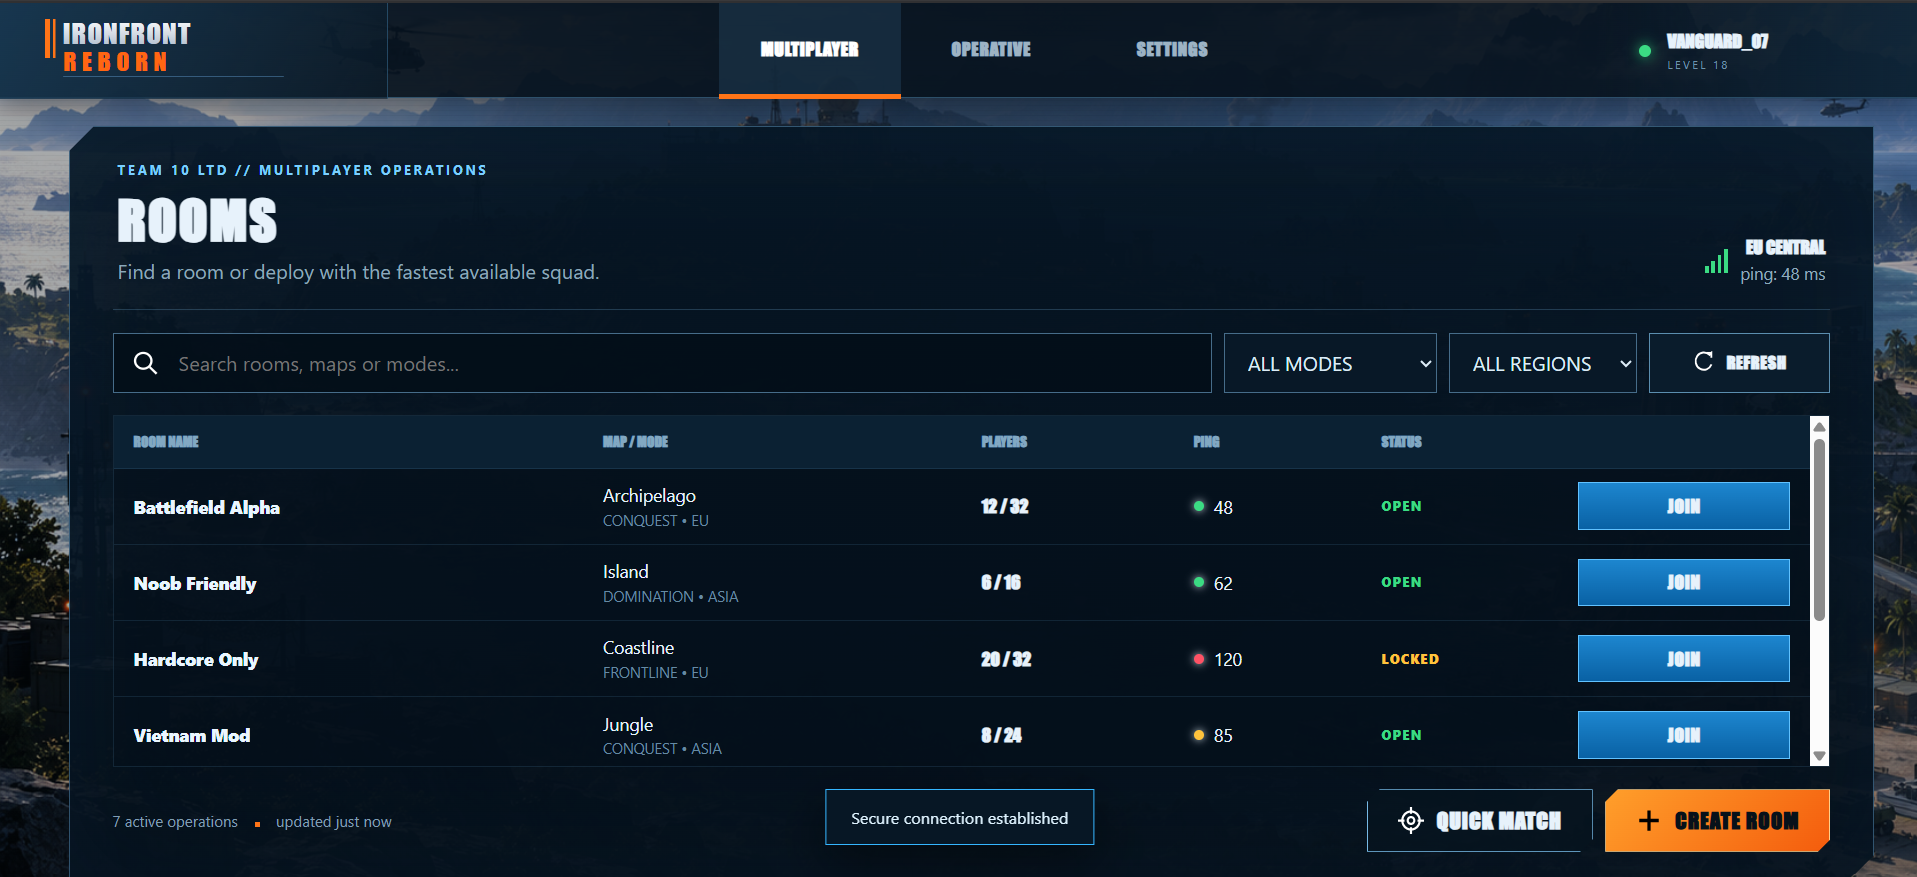
\includegraphics[width=0.9\textwidth]{image/room-browser.png}
\caption{Danh sách phòng (trạng thái \texttt{RoomBrowser}): tìm kiếm, lọc theo chế độ và khu vực, làm mới, vào
phòng, ghép trận nhanh và tạo phòng}
\label{fig:A-sanh}
\end{figure}

\begin{figure}[H]
\centering
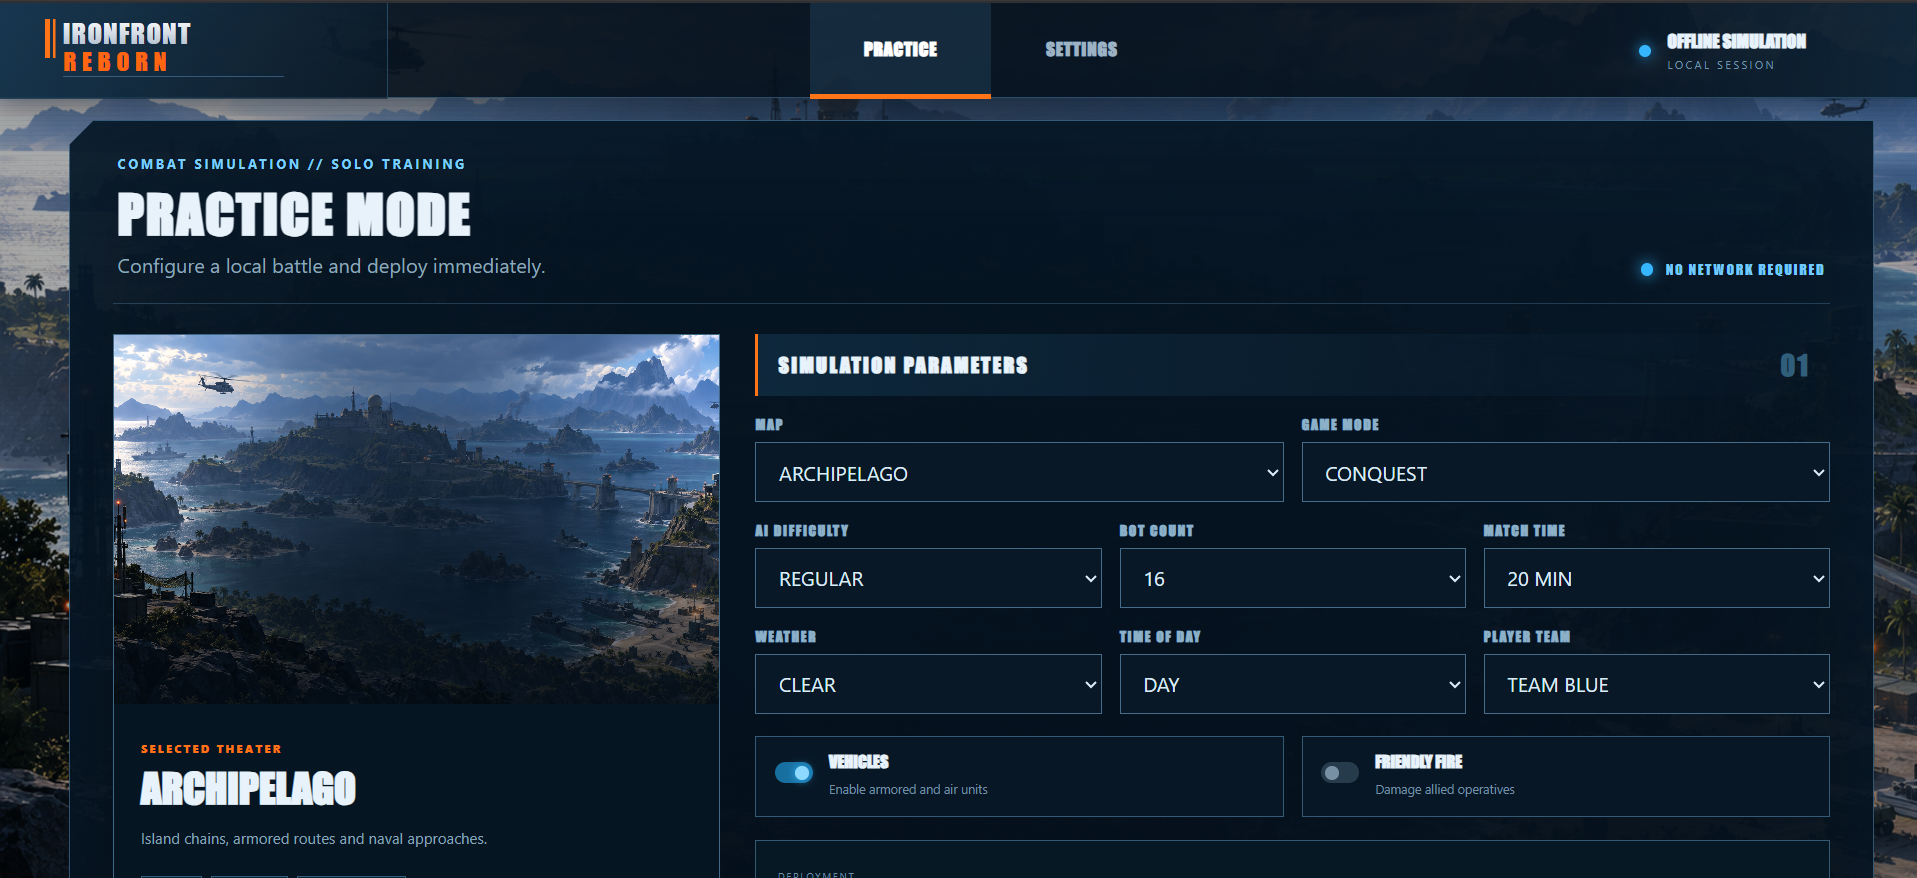
\includegraphics[width=0.9\textwidth]{image/practice-mode.png}
\caption{Màn hình luyện tập ngoại tuyến: chọn bản đồ, chế độ chơi, độ khó và số lượng bot, không cần kết nối mạng}
\label{fig:A-luyentap}
\end{figure}

\begin{figure}[H]
\centering

\includegraphics[width=0.9\textwidth]{image/settings.png}
\caption{Màn hình cài đặt: hiển thị, âm thanh và lối chơi, lưu theo máy}
\label{fig:A-caidat}
\end{figure}

% -------------------------------------------------------------------------------------
\subsection{Giao diện trong trận và overlay chẩn đoán}
\begin{figure}[H]
\centering
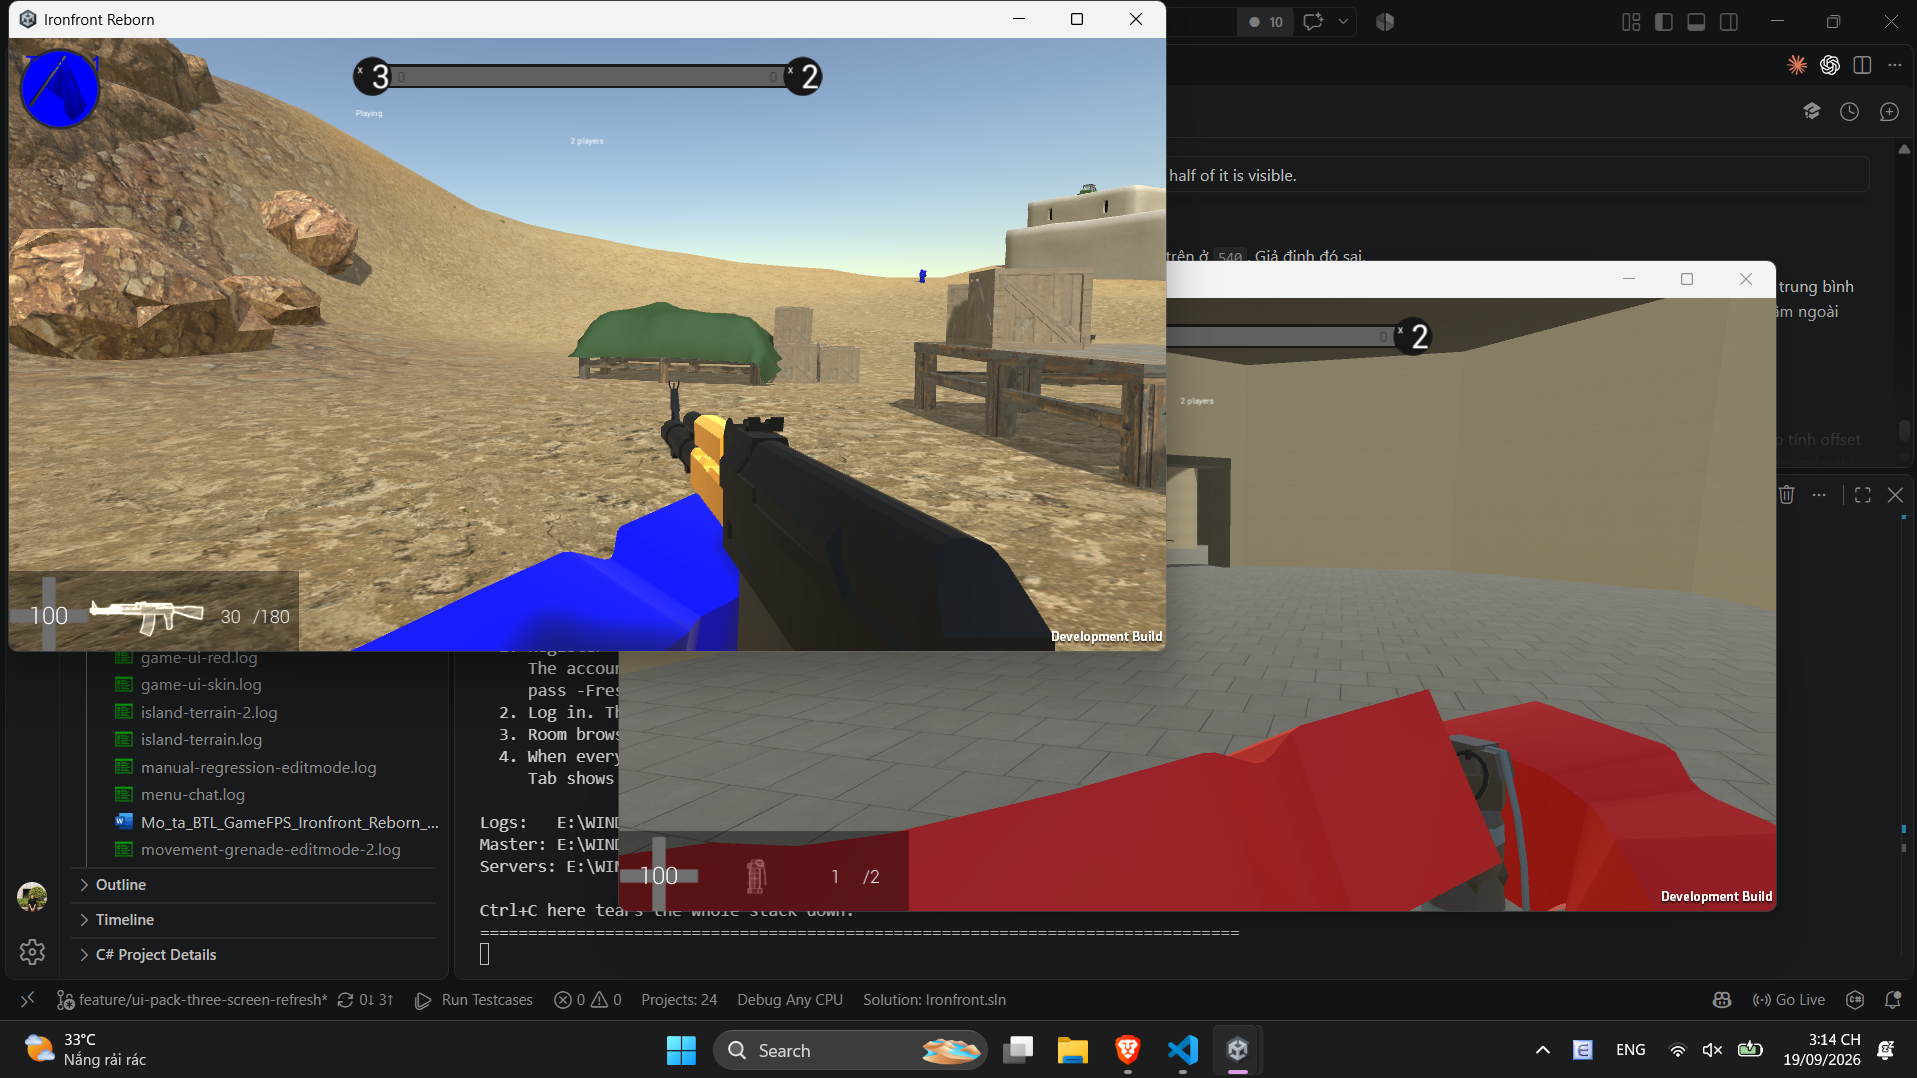
\includegraphics[width=0.9\textwidth]{image/ingame.png}
\caption{Màn hình trong trận đấu}
\label{fig:A-hud}
\end{figure}

% -------------------------------------------------------------------------------------
\subsection{Luồng dự đoán và hoà giải phía client}
\begin{figure}[H]
\centering
\begin{tikzpicture}[x=1cm, y=1cm]
  \node[bxB, text width=2.5cm] (t)  at (1.45,0)   {NetPrediction\\Clock\\{\footnotesize bước 30 Hz}};
  \node[bxB, text width=2.4cm] (i)  at (4.6,0)   {LocalInputSource\\{\footnotesize InputFrame(tick)}};
  \node[bxG, text width=2.6cm] (m)  at (7.9,0)   {NetMovementAgent\\{\footnotesize mô phỏng ngay}};
  \node[bxB, text width=2.3cm] (q)  at (11.1,0)  {Lưu input\\chưa xác nhận};
  \node[bxP, text width=2.2cm] (s)  at (14.3,0)  {C\_INPUT kênh 3\\{\footnotesize tối đa 8 frame}};
  \node[grp, fit=(t)(s)] (g1) {};
  \node[grpt] at (g1.north west) {1. Dự đoán - mỗi tick};
  \draw[arr] (t) -- (i); \draw[arr] (i) -- (m); \draw[arr] (m) -- (q); \draw[arr] (q) -- (s);

  \node[bxP, text width=2.5cm] (n)  at (1.6,-2.9) {S\_SNAPSHOT\\{\footnotesize ClientMessageRouter}};
  \node[bxB, text width=3.1cm] (h)  at (5.4,-2.9) {SnapshotHolding\\Queue};
  \node[bxG, text width=3.2cm] (r)  at (9.2,-2.9) {PredictionReconciler\\{\footnotesize so tại lastProcessedInputTick}};
  \node[bxO, text width=3.0cm] (c)  at (13.4,-2.9) {Lệch quá ngưỡng: đặt về server, phát lại input};
  \node[grp, fit=(n)(c)] (g2) {};
  \node[grpt] at (g2.north west) {2. Hoà giải - khi có snapshot mới};
  \draw[arr] (n) -- (h); \draw[arr] (h) -- (r); \draw[arr] (r) -- (c);
  \draw[darr] (q.south) -- node[lbl, right=2pt]{input chưa xác nhận} (q.south |- r.north);

  \node[bxB, text width=3.0cm] (ri) at (3.2,-5.8) {RemoteActorRegistry};
  \node[bxG, text width=3.4cm] (si) at (7.9,-5.8) {SnapshotInterpolator\\{\footnotesize hiển thị tại now $-$ 100 ms}};
  \node[bxG, text width=3.2cm] (rv) at (12.6,-5.8) {RemoteActorView\\{\footnotesize tư thế, vũ khí, hoạt ảnh}};
  \node[grp, fit=(ri)(rv)] (g3) {};
  \node[grpt] at (g3.north west) {3. Nội suy actor ở xa};
  \draw[arr] (ri) -- (si); \draw[arr] (si) -- (rv);
  \draw[arr] (h.south) -- node[lbl, right=2pt]{actor ở xa} (h.south |- ri.north);
\end{tikzpicture}
\caption{Luồng xử lý dự đoán, hoà giải và nội suy trong client}
\label{fig:A-duDoan}
\end{figure}

% =====================================================================================
\section{Luồng xử lý và giải pháp đã ứng dụng}
Mục này mô tả chi tiết các luồng mà phân hệ client hiện thực: từ màn hình đăng nhập tới sảnh, vào phòng và kết nối
game server bằng vé, rồi trong trận là dự đoán - hoà giải chuyển động của người chơi cục bộ, nội suy người chơi ở xa,
hiển thị sự kiện chiến đấu và HUD, cuối cùng là mất kết nối và kết thúc trận.

% -------------------------------------------------------------------------------------
\subsection{Luồng đăng nhập từ giao diện}
\textbf{Bài toán.} Luồng dựng giao diện chạy trên luồng chính của client; nếu dừng chờ phản hồi mạng đồng bộ thì giao diện sẽ bị treo đóng băng. Ngược lại, các sự kiện nhận dữ liệu mạng chạy từ luồng nền không được phép trực tiếp thao tác lên cây đối tượng hiển thị.

\begin{figure}[H]
\centering
\renewcommand{\seqstep}{0.64cm}
\begin{tikzpicture}[x=1cm, y=1cm]
  \seqhuman{P}{0.6}{Người chơi}
  \seqactor{O}{3.5}{Giao diện\\sảnh chờ}
  \seqactor{S}{6.9}{Phiên kết nối\\Master}
  \seqactor{F}{10.2}{Bộ điều phối\\luồng game}
  \seqactor{M}{13.4}{Client TCP\\Master}
  \seqactor{X}{15.9}{Máy chủ\\Master}
  \seqbegin
  \seqmsg{P}{O}{Nhập máy chủ, tài khoản, mật khẩu; bấm ``Đăng nhập''}
  \seqmsg{O}{S}{Yêu cầu xử lý đăng nhập bất đồng bộ}
  \seqmsg{S}{M}{Khởi tạo kết nối TCP bảo mật (TLS)}
  \seqmsg{M}{X}{TCP + bắt tay mã hoá TLS}
  \seqmsg{S}{F}{Chuyển trạng thái: Đang xác thực}
  \seqself{S}{Băm bảo mật phía client:\\SHA256(mật khẩu + username)}
  \seqmsg{S}{M}{Gửi bản tin đăng nhập kèm mã băm}
  \seqmsg{M}{X}{LOGIN\_REQ (trên luồng nền)}
  \seqret{X}{M}{LOGIN\_RES}
  \seqself{M}{Đưa phản hồi vào hàng đợi an toàn luồng;\\xử lý trên luồng chính của client}
  \seqfragbegin
  \seqret{M}{S}{Thành công: phiên kết nối, mã người chơi, tên hiển thị}
  \seqmsg{S}{F}{Chuyển trạng thái: Sảnh chờ}
  \seqfragelse{P}{X}{Lỗi (sai mật khẩu, bị khoá tạm thời, quá tần suất, sai phiên bản)}
  \seqret{M}{S}{Thông báo lỗi xác thực}
  \seqmsg{S}{F}{Phục hồi về màn hình đăng nhập}
  \seqfragend{P}{X}{alt}{Đăng nhập thành công}
  \seqret{O}{P}{Cập nhật giao diện; hiển thị câu thông báo lỗi thân thiện}
  \seqend{P,O,S,F,M,X}
\end{tikzpicture}
\caption{Biểu đồ tuần tự đăng nhập: giao diện không bao giờ chặn, mọi kết quả về luồng chính an toàn}
\label{fig:A-luong-dangnhap}
\end{figure}

\begin{center}\small
\begin{tabularx}{\linewidth}{|L{4.4cm}|Y|}
\hline
\hd{Vấn đề} & \hd{Giải pháp đã áp dụng} \\ \hline
Giao diện không thể dừng chờ mạng & Xử lý mạng bất đồng bộ có khối bắt lỗi bao trọn, bảo đảm ngoại lệ không thoát ra làm gián đoạn luồng chính \\ \hline
Sự kiện mạng chạy trên luồng nền & Sử dụng hàng đợi an toàn luồng để chuyển dữ liệu từ luồng nhận sang xử lý tại luồng giao diện ở mỗi khung hình \\ \hline
Chuyển màn hình sai thứ tự khi thao tác chồng nhau & Quản lý bằng máy trạng thái 10 trạng thái có bảng chuyển dịch hợp lệ; mọi thao tác sai luồng đều bị từ chối và kích hoạt quy trình phục hồi \\ \hline
Mật khẩu lộ ra đường truyền hoặc log máy chủ & Băm SHA-256 kết hợp tên người dùng ngay tại client trước khi truyền; mật khẩu phòng cũng được băm độc lập \\ \hline
Mã lỗi kỹ thuật khó hiểu & Bảng ánh xạ mã lỗi hệ thống sang thông điệp tiếng Việt thân thiện, rõ ràng cho người chơi \\ \hline
\end{tabularx}
\end{center}

% -------------------------------------------------------------------------------------
\subsection{Luồng vào phòng và kết nối game server}
\begin{figure}[H]
\centering
\renewcommand{\seqstep}{0.64cm}
\begin{tikzpicture}[x=1cm, y=1cm]
  \seqactor{S}{1.2}{Phiên Master}
  \seqactor{F}{4.5}{Bộ điều phối\\luồng game}
  \seqactor{Q}{7.8}{Hàng đợi giữ\\Snapshot}
  \seqactor{T}{11.3}{Client giao vận\\UDP}
  \seqactor{G}{14.8}{Game Server}
  \seqbegin
  \seqmsg{S}{F}{Chuyển trạng thái: Đang vào phòng}
  \seqself{S}{Yêu cầu vào phòng kèm hash mật khẩu phòng}
  \seqself{S}{Lưu thông tin kết nối và vé xác thực}
  \seqmsg{S}{F}{Chuyển trạng thái: Sảnh phòng}
  \seqmsg{S}{F}{Bắt đầu vào trận: Đang kết nối game}
  \seqmsg{S}{Q}{Kích hoạt chế độ giữ gói snapshot đến}
  \seqmsg{S}{T}{Khởi tạo kết nối UDP với vé tham gia}
  \seqmsg{T}{G}{CONNECT\_REQUEST / RESPONSE (bắt tay cookie)}
  \seqfragbegin
  \seqret{G}{T}{CONNECT\_ACCEPTED \{mã kết nối, tick server, bản đồ\}}
  \seqret{T}{S}{Kết nối thành công: Tải scene bản đồ}
  \seqmsg{T}{Q}{S\_MATCH\_STATE, S\_SPAWN\_ACTOR, S\_SNAPSHOT (giữ lại)}
  \seqmsg{S}{Q}{Bản đồ tải xong: Giải phóng và xử lý gói đã giữ}
  \seqmsg{S}{F}{Chuyển trạng thái: Trong trận đấu}
  \seqfragelse{S}{G}{Quá 10 s hoặc CONNECT\_DENIED}
  \seqself{S}{Ghi nhận lỗi kết nối}
  \seqmsg{S}{F}{Phục hồi về sảnh phòng}
  \seqfragend{S}{G}{alt}{Được chấp nhận}
  \seqend{S,F,Q,T,G}
\end{tikzpicture}
\caption{Biểu đồ tuần tự từ vào phòng tới vào trận: vé từ master, bắt tay UDP, giữ gói trong lúc tải bản đồ}
\label{fig:A-luong-vaotran}
\end{figure}

\textbf{Các giải pháp kỹ thuật chính.}
\begin{itemize}
  \item \textbf{Gói trọn địa chỉ, cổng và vé vào một cấu trúc dữ liệu duy nhất.} Tránh việc gọi nhầm server này với vé của server khác (game server sẽ từ chối với lỗi chữ ký không nói rõ nguyên nhân). Vé chỉ sống 60 s nên client kết nối ngay và hết hạn chờ sau 10 s - nằm gọn trong hạn của vé.
  \item \textbf{Giữ gói trong lúc tải bản đồ.} Server bắt đầu gửi trạng thái ngay sau khi chấp nhận kết nối, khi bản đồ còn đang tải. Hàng đợi giữ snapshot bắt đầu kích hoạt \textbf{trước} khi gửi gói kết nối, và chỉ phát lại khi bản đồ sẵn sàng; vì thế không có khoảng hở nào để một gói bị đưa vào đối tượng chưa tồn tại.
  \item \textbf{Xử lý lỗi kết nối an toàn.} Vé sai định dạng, cổng ngoài phạm vi hay địa chỉ không phân giải được đều được xử lý an toàn thành thông báo và trạng thái tự động quay về sảnh phòng.
  \item \textbf{Kết nối trực tiếp không cần master:} Hỗ trợ chế độ kết nối trực tiếp sử dụng vé mặc định dành riêng cho việc kiểm thử độc lập trong mạng cục bộ.
\end{itemize}

% -------------------------------------------------------------------------------------
\subsection{Luồng dự đoán và hoà giải chuyển động người chơi cục bộ}
\begin{figure}[H]
\centering
\renewcommand{\seqstep}{0.64cm}
\begin{tikzpicture}[x=1cm, y=1cm]
  \seqactor{K}{1.3}{Đồng hồ\\dự đoán}
  \seqactor{A}{4.7}{Tác nhân\\chuyển động}
  \seqactor{P}{8.2}{Tầng dự đoán\\client}
  \seqactor{R}{11.8}{Bộ đối soát\\hoà giải}
  \seqactor{T}{15.0}{Giao vận\\(kênh 3)}
  \seqbegin
  \seqfragbegin
  \seqmsg{K}{A}{Mô phỏng bước di chuyển (chu kỳ 1/30 s)}
  \seqself{A}{Thuật toán mô phỏng đồng nhất với server}
  \seqmsg{K}{P}{Ghi nhận tick vừa mô phỏng}
  \seqmsg{P}{R}{Lưu trữ input vào bộ đệm vòng tròn}
  \seqmsg{P}{T}{C\_INPUT \{tick cũ nhất, tối đa 8 frame\} - không tin cậy}
  \seqfragend{K}{T}{loop}{mỗi tick 30 Hz}
  \seqret{T}{P}{Nhận snapshot từ server kèm tick input đã xử lý}
  \seqmsg{P}{R}{Đối soát vị trí dự đoán với vị trí server}
  \seqfragbegin
  \seqret{R}{P}{Khớp vị trí: không điều chỉnh}
  \seqfragelse{K}{T}{Lệch vượt ngưỡng 0,25 m}
  \seqself{R}{Nhận vị trí chuẩn từ server,\\sau đó phát lại các input chưa được xác nhận}
  \seqret{R}{P}{Đã sửa sai vị trí}
  \seqfragelse{K}{T}{Input phát lại đã bị đẩy khỏi vòng đệm}
  \seqret{R}{P}{Đồng bộ cưỡng bức: đặt thẳng về vị trí server}
  \seqfragend{K}{T}{alt}{Lệch $\le$ 0,25 m}
  \seqmsg{P}{A}{Cập nhật vị trí chuẩn xác vào nhân vật}
  \seqend{K,A,P,R,T}
\end{tikzpicture}
\caption{Biểu đồ tuần tự dự đoán phía client và hoà giải với snapshot của server}
\label{fig:A-luong-dudoan}
\end{figure}

\begin{center}\small
\begin{tabularx}{\linewidth}{|L{4.4cm}|Y|}
\hline
\hd{Vấn đề} & \hd{Giải pháp đã áp dụng} \\ \hline
Chờ server trả lời mới di chuyển thì trễ bằng một vòng RTT & Dự đoán: mô phỏng ngay tại client bằng cùng thuật toán vật lý với server nên cùng input cho cùng kết quả \\ \hline
Gói input bị mất & Mỗi gói mang tối đa 8 frame gần nhất (266 ms dư thừa ở 30 Hz), gửi không tin cậy trên kênh 3 - rẻ hơn trả ack cho 30 bản tin mỗi giây \\ \hline
Dự đoán lệch server & So sánh tại tick input gần nhất server đã xử lý; lệch quá 0,25 m thì \textbf{nhận trạng thái server trước rồi mới phát lại} input chưa xác nhận (phát lại lên trạng thái dự đoán sẽ nhân đôi sai số) \\ \hline
Ghi input sai tick làm mọi lần phát lại lệch khung & Lưu input vào bộ đệm \textbf{trước} khi gửi và dùng đúng số tick mà đồng hồ đã đóng dấu \\ \hline
Số thứ tự tick quay vòng & So sánh bằng số học modulo tuần hoàn; dữ liệu cũ bị loại bỏ \\ \hline
Cập nhật vị trí nhân vật quá nhiều & Chỉ cập nhật lại vị trí nhân vật khi có sự sai lệch vị trí vượt ngưỡng quy định \\ \hline
\end{tabularx}
\end{center}

% -------------------------------------------------------------------------------------
\subsection{Luồng hiển thị người chơi và bot ở xa}
\begin{figure}[H]
\centering
\renewcommand{\seqstep}{0.64cm}
\begin{tikzpicture}[x=1cm, y=1cm]
  \seqactor{R}{1.3}{Bộ định tuyến\\thông điệp}
  \seqactor{G}{4.9}{Quản lý nhân vật\\ở xa}
  \seqactor{I}{8.7}{Bộ nội suy\\Snapshot}
  \seqactor{V}{12.3}{Giao diện hiển thị\\nhân vật ở xa}
  \seqactor{U}{15.4}{Nhân vật\\đồ hoạ}
  \seqbegin
  \seqmsg{R}{G}{Thông báo tạo nhân vật mới (S\_SPAWN\_ACTOR)}
  \seqmsg{G}{V}{Khởi tạo và gán đối tượng hiển thị theo ID}
  \seqfragbegin
  \seqmsg{R}{I}{Lưu trữ snapshot thế giới đã giải nén delta}
  \seqfragend{R}{U}{loop}{mỗi gói S\_SNAPSHOT}
  \seqfragbegin
  \seqmsg{G}{I}{Lấy mẫu nội suy (thời điểm trễ 100 ms)}
  \seqret{I}{G}{Điểm đầu, điểm đích, hệ số nội suy}
  \seqmsg{G}{V}{Áp dụng vị trí, hướng nhìn, tư thế, vũ khí}
  \seqmsg{V}{U}{Điều khiển hình thể, hoạt ảnh và hiệu ứng}
  \seqfragend{R}{U}{loop}{mỗi khung hình hiển thị}
  \seqmsg{R}{G}{Thông báo huỷ nhân vật (S\_DESPAWN\_ACTOR)}
  \seqmsg{G}{V}{Gỡ bỏ đối tượng hiển thị, thu hồi tài nguyên}
  \seqend{R,G,I,V,U}
\end{tikzpicture}
\caption{Biểu đồ tuần tự nội suy actor ở xa giữa hai snapshot đã nhận}
\label{fig:A-luong-noisuy}
\end{figure}

\textbf{Giải pháp.} Snapshot chỉ tới 20 Hz (xa hơn còn 10 hoặc 4 Hz) nên hiển thị thẳng sẽ giật. Client hiển thị lùi sau snapshot mới nhất 2 tick và \textbf{nội suy} giữa hai snapshot bao quanh thời điểm đó - mất một snapshot vẫn còn cặp khác để nội suy, đúng yêu cầu ``chuyển động của người khác luôn mượt khi mất gói''. Vòng đệm 16 snapshot (nửa giây) được cấp phát một lần; snapshot được sao chép vào bộ đệm nội suy riêng biệt. Nếu thời điểm hiển thị cũ hơn snapshot cũ nhất thì dừng ở snapshot cũ nhất chứ không ngoại suy lùi. Hiệu ứng gục ngã khi chết chỉ là hiệu ứng cục bộ, không đồng bộ (tiết kiệm băng thông đáng kể).

% -------------------------------------------------------------------------------------
\subsection{Luồng sự kiện chiến đấu, mục tiêu và HUD}
\begin{figure}[H]
\centering
\renewcommand{\seqstep}{0.64cm}
\begin{tikzpicture}[x=1cm, y=1cm]
  \seqactor{T}{1.3}{Giao vận\\(kênh 1, 2)}
  \seqactor{R}{4.7}{Bộ định tuyến\\thông điệp}
  \seqactor{C}{8.4}{Bộ hiển thị\\chiến đấu}
  \seqactor{O}{12.1}{Bộ hiển thị\\mục tiêu}
  \seqactor{H}{15.3}{Giao diện HUD /\\hiệu ứng}
  \seqbegin
  \seqmsg{T}{R}{Payload dữ liệu hoàn chỉnh}
  \seqfragbegin
  \seqmsg{R}{C}{S\_WEAPON\_FIRE}
  \seqmsg{C}{H}{Âm thanh khai hoả, hiệu ứng vệt đạn}
  \seqfragelse{T}{H}{S\_HIT\_CONFIRM}
  \seqmsg{R}{C}{S\_HIT\_CONFIRM \{mã mục tiêu, sát thương\}}
  \seqmsg{C}{H}{Hiệu ứng trúng đích (hitmarker), âm thanh trúng}
  \seqfragelse{T}{H}{S\_DEATH}
  \seqmsg{R}{C}{S\_DEATH \{nạn nhân, người bắn, vũ khí\}}
  \seqmsg{C}{H}{Thông báo hạ gục, hiệu ứng gục ngã, đếm ngược hồi sinh}
  \seqfragelse{T}{H}{S\_MATCH\_STATE / S\_CAPTURE\_POINT}
  \seqmsg{R}{O}{Pha trận, số vé mỗi phe, trạng thái cứ điểm}
  \seqmsg{O}{H}{Cập nhật thanh vé, cờ cứ điểm, bảng điểm trận đấu}
  \seqfragend{T}{H}{alt}{S\_WEAPON\_FIRE}
  \seqend{T,R,C,O,H}
\end{tikzpicture}
\caption{Biểu đồ tuần tự biến sự kiện server thành hiệu ứng và HUD}
\label{fig:A-luong-sukien}
\end{figure}
Máu, đạn, hạ gục và điểm số đều \textbf{do server quyết định}; client chỉ hiển thị. Giật súng cục bộ vẫn chạy để có cảm giác
bắn, nhưng không ảnh hưởng viên đạn thật. Trước khi áp dụng lên đối tượng, mọi bộ hiển thị kiểm tra hai điều kiện: ``có phải vai trò client mạng không'' và ``đối tượng có phải người đang ngồi trước máy không'' - để hiệu ứng dành riêng cho người chơi (dấu trúng đạn, đếm ngược hồi sinh) không bị áp nhầm lên nhân vật khác ở xa.

% -------------------------------------------------------------------------------------
\subsection{Luồng mất kết nối và kết thúc trận}
Theo đề, hết trận server hiện bảng điểm 20 s rồi đặt lại thế giới, người chơi không phải thoát phòng; còn người chơi mất
kết nối quá 10 s bị coi như rời trận. Phía client xử lý hai trường hợp như sau.
\begin{figure}[H]
\centering
\renewcommand{\seqstep}{0.64cm}
\begin{tikzpicture}[x=1cm, y=1cm]
  \seqactor{T}{1.4}{Client giao vận\\UDP}
  \seqactor{S}{5.6}{Phiên Master}
  \seqactor{F}{9.8}{Bộ điều phối\\luồng game}
  \seqhuman{P}{14.2}{Người chơi}
  \seqbegin
  \seqfragbegin
  \seqmsg{T}{S}{Thông báo mất kết nối (Hết thời gian chờ / Lỗi mạng)}
  \seqself{S}{Ghi nhận sự cố mất kết nối với game server}
  \seqmsg{S}{F}{Chuyển trạng thái phục hồi về Sảnh chờ}
  \seqret{F}{P}{Quay về sảnh kèm thông báo, không bị treo ứng dụng}
  \seqfragelse{T}{P}{S\_MATCH\_STATE: Chuyển pha kết thúc trận}
  \seqret{T}{P}{HUD hiển thị bảng điểm, thời gian chờ vòng tiếp theo}
  \seqret{T}{P}{Bắt đầu vòng mới: S\_SPAWN\_ACTOR, tiếp tục trận đấu}
  \seqfragend{T}{P}{alt}{Mất kết nối giữa trận}
  \seqend{T,S,F,P}
\end{tikzpicture}
\caption{Biểu đồ tuần tự phía client khi mất kết nối và khi trận kết thúc}
\label{fig:A-luong-roi}
\end{figure}
Khi server không nhận được gói nào trong 10 s, nó coi người chơi đã rời trận; phía client cũng tự hết hạn sau 10 s im lặng và
đưa người chơi về sảnh với thông báo, thay vì để lại một thế giới đứng yên không ai cập nhật.

% -------------------------------------------------------------------------------------
\subsection{Bảng ánh xạ hình vẽ với chức năng cá nhân thực hiện}
\label{sec:A-mapping-hinh-ve}
Bảng tổng hợp đối chiếu toàn bộ các sơ đồ kiến trúc, giao diện và luồng xử lý do cá nhân thực hiện tương ứng với các chức năng cụ thể trong phân hệ client Unity:

\begin{center}\small
\begin{tabularx}{\linewidth}{|L{2.2cm}|L{4.2cm}|Y|}
\hline
\hd{Hình vẽ} & \hd{Tên hình vẽ / biểu đồ} & \hd{Chức năng cá nhân thực hiện} \\ \hline
Hình~\ref{fig:A-lop} & Biểu đồ cấu trúc lớp điểm nối & Trừu tượng hoá và tách biệt nguồn dữ liệu điều khiển nhân vật khỏi logic hiển thị; hỗ trợ đa nguồn input (bàn phím chuột, gói mạng UDP từ server hoặc bot AI). \\ \hline
Hình~\ref{fig:A-thutu} & Thứ tự thực thi khung hình & Thiết lập chu trình thực thi các thành phần mạng client theo thứ tự ưu tiên: nhận và giải mã gói tin trước, cập nhật hiển thị sau, tránh hiện tượng lệch frame. \\ \hline
Hình~\ref{fig:A-trangthai} & Máy trạng thái luồng game & Quản lý máy trạng thái 10 trạng thái toàn cục của client; chặn mọi chuyển đổi trạng thái bất hợp lệ và bảo đảm quy trình phục hồi an toàn khi lỗi mạng. \\ \hline
Hình~\ref{fig:A-menu} & Màn hình chính & Xây dựng giao diện menu chính: điều hướng chế độ chơi mạng (Multiplayer), luyện tập offline, thiết lập cài đặt và thoát trò chơi. \\ \hline
Hình~\ref{fig:A-dangnhap} & Màn hình đăng nhập & Thiết kế biểu mẫu nhập thông tin, xử lý băm mật khẩu bảo mật tại máy khách và hiển thị thông báo lỗi phản hồi từ máy chủ trung tâm. \\ \hline
Hình~\ref{fig:A-sanh} & Danh sách phòng chơi & Hiện thực giao diện sảnh chờ: tìm kiếm phòng, lọc phòng theo chế độ/khu vực, hiển thị danh sách phòng trực quan, tạo phòng và ghép trận nhanh. \\ \hline
Hình~\ref{fig:A-luyentap} & Màn hình luyện tập & Xây dựng tính năng luyện tập ngoại tuyến: chọn bản đồ, tuỳ chỉnh số lượng bot AI, chế độ chơi mà không cần kết nối mạng. \\ \hline
Hình~\ref{fig:A-caidat} & Màn hình cài đặt & Thiết kế hệ thống cài đặt client: cấu hình hiển thị đồ họa, âm lượng và độ nhạy chuột, lưu trữ cấu hình cục bộ theo máy. \\ \hline
Hình~\ref{fig:A-hud} & Giao diện HUD trong trận & Tích hợp giao diện HUD chiến đấu: thanh máu, lượng đạn, la bàn định hướng, tiến độ điểm chiếm, bảng điểm và hiệu ứng phản hồi trúng đạn. \\ \hline
Hình~\ref{fig:A-duDoan} & Sơ đồ xử lý dự đoán và nội suy & Thiết kế kiến trúc xử lý kép: mô phỏng dự đoán cục bộ phản hồi tức thời kết hợp bộ đệm nội suy mượt mà đối với người chơi ở xa. \\ \hline
Hình~\ref{fig:A-luong-dangnhap} & Sơ đồ tuần tự đăng nhập & Hiện thực luồng đăng nhập bất đồng bộ: không chặn luồng giao diện, băm SHA-256 mật khẩu và chuyển kết quả an toàn về luồng chính. \\ \hline
Hình~\ref{fig:A-luong-vaotran} & Sơ đồ tuần tự vào trận & Hiện thực luồng vào phòng, nhận vé xác thực 64 byte từ master, bắt tay UDP với game server và lưu đệm gói tin khi đang tải bản đồ. \\ \hline
Hình~\ref{fig:A-luong-dudoan} & Sơ đồ tuần tự dự đoán & Hiện thực thuật toán dự đoán di chuyển 30 Hz phía client, lưu trữ bộ đệm input và hoà giải sai lệch vị trí khi nhận snapshot chuẩn từ server. \\ \hline
Hình~\ref{fig:A-luong-noisuy} & Sơ đồ tuần tự nội suy & Hiện thực thuật toán lấy mẫu nội suy giữa hai snapshot lịch sử (lùi 100 ms), đảm bảo hiển thị mượt mà ngay cả khi mất gói mạng. \\ \hline
Hình~\ref{fig:A-luong-sukien} & Sơ đồ tuần tự sự kiện & Tiếp nhận và giải mã các sự kiện chiến đấu có thẩm quyền từ server; kích hoạt âm thanh, dấu trúng đạn (hitmarker) và cập nhật thanh điểm. \\ \hline
Hình~\ref{fig:A-luong-roi} & Sơ đồ tuần tự rời trận & Xử lý tự động hết thời gian chờ ngắt kết nối (10 s im lặng), bảo vệ trò chơi không bị treo cứng và quay trở lại sảnh chờ an toàn. \\ \hline
\end{tabularx}
\end{center}
